\documentclass[10pt]{article}
\usepackage[margin=0.5in]{geometry}
\usepackage{amsmath,amssymb}
\usepackage{graphicx}
\usepackage{subfig}
\usepackage{float}
\usepackage{makecell}
\usepackage{listings}
\begin{document}
{\centering
CS7CS4 Machine Learning - Week 3
\par
Arnav Bhattacharya - 22307812
\par
Dataset \# id:15--15--15
\par
}
\vspace{5mm}
\begin{center}
  \textbf{Appendix contains all code for all questions and their respective subparts.}
\end{center}

\section*{Question i}
\textbf{In this assignment you'll use sklearn to train and evaluate Lasso regression models on the
  data you downloaded. Recall that Lasso regression uses a linear model and mean square
  cost function with an L1 penalty and that the L1 penalty has a weight parameter C in the
  lecture notes (weight parameter {\begin{equation*} \alpha = \dfrac {1}{2C} \end{equation*}} in sklearn).}

\subsection*{Part a}
\textbf{Plot the data you downloaded as a 3D scatter plot i.e. with the first feature on
  the x-axis, the second feature in the y-axis and the target on the z-axis. You
  can use the matplotlib scatter function for this, e..g for training data with two
  features X and target y.
}

\begin{center}
  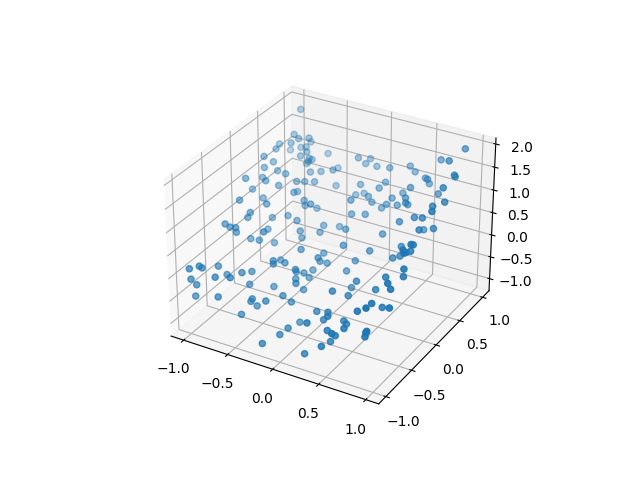
\includegraphics[scale=0.4]{./images/Figure_1.png}
\end{center}

If the graph is viewed from all the angles(180\textdegree and 360\textdegree respectively as shown in the images below), we can see that all the points lie on a curve and not on a plane. Also, when we view the dispersion [dispersion:  3.6094470441670876] from the normal axis, we see that the resulting value is high. Hence, the points lie on a curve.

\begin{figure}[hbt!]
  \begin{center}
    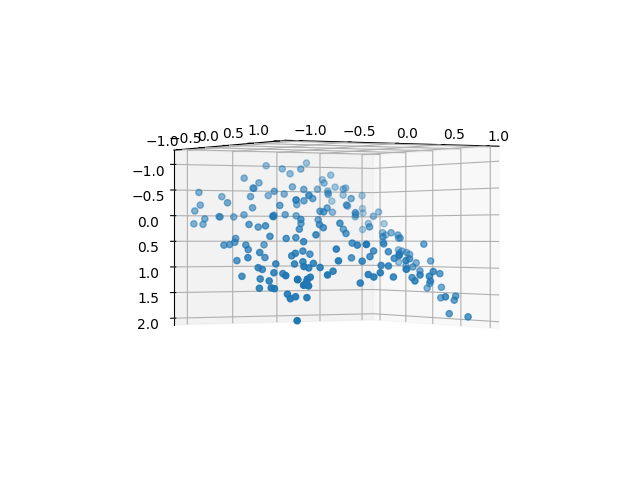
\includegraphics[scale=0.4]{./images/Figure_1_180.png}
    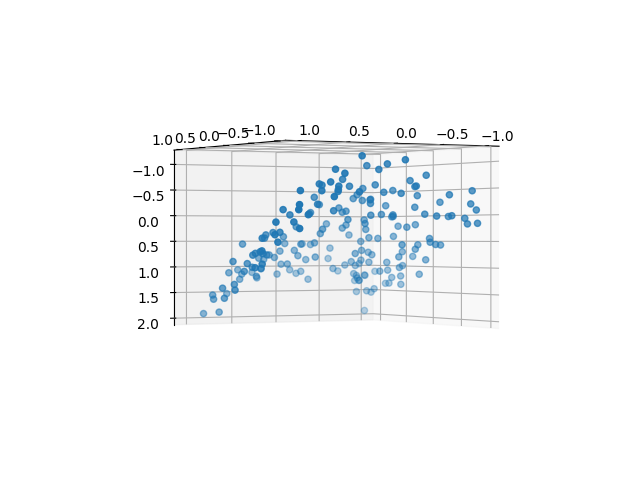
\includegraphics[scale=0.4]{./images/Figure_1_360.png}
    \caption{Dataset Visualization after rotating 180\textdegree and 360\textdegree respectively}
  \end{center}
\end{figure}
\vspace{10mm}

\subsection*{Part b}
\textbf{In addition to the two features in the data file add extra polynomial features
  equal to all combinations of powers of the two features up to power 5 (you
  can use the sklearn PolynomialFeatures function to do this). Now train Lasso
  regression models with these polynomial features for a large range of values of
  C e.g. 1, 10, 1000 (you might need to adjust these values for your data, start
  by making C small enough that the trained model has all parameters zero, then
  increase from there). Report the parameters of the trained models (don't just
  give a list of numbers, say what feature each parameter value corresponds to),
  discuss how they change as C is varied.}

Lasso regression uses a linear model and mean square cost function with an L1 penalty
and that the L1 penalty has a weight parameter C. Lasso regression models were trained
on the data set provided along with the polynomial features equal to all combinations of
powers of the two features up to power 5. I used PolynomialFeatures function from sklearn package.
Lasso regression models were trained on the data for a large number of penalty values, specifically,
[1, 5, 10, 50, 100, 500, 1000] values.

\begin{center}
  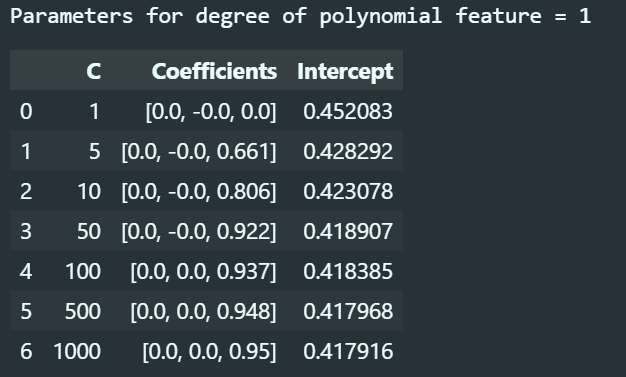
\includegraphics[scale=0.4]{./images/Table_1.png}
  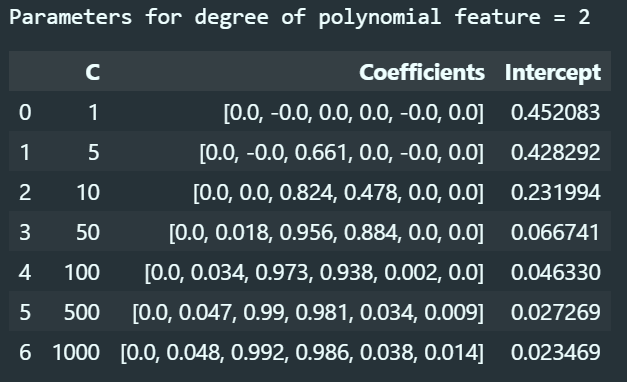
\includegraphics[scale=0.4]{./images/Table_2.png}
  \vspace{5mm}
  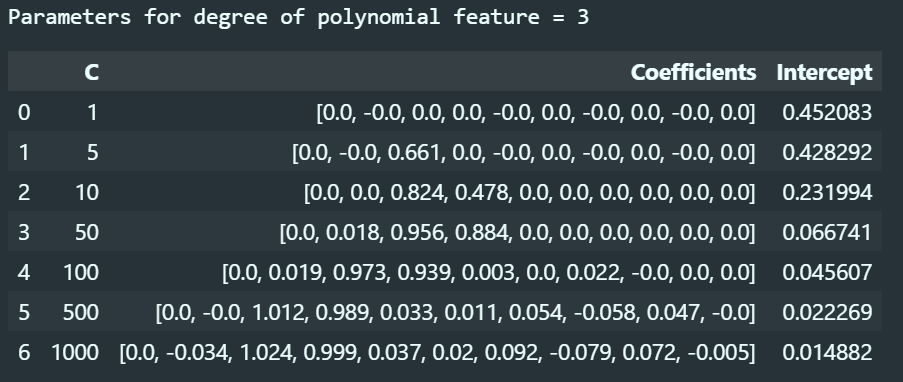
\includegraphics[scale=0.4]{./images/Table_3.png}
  \vspace{5mm}
  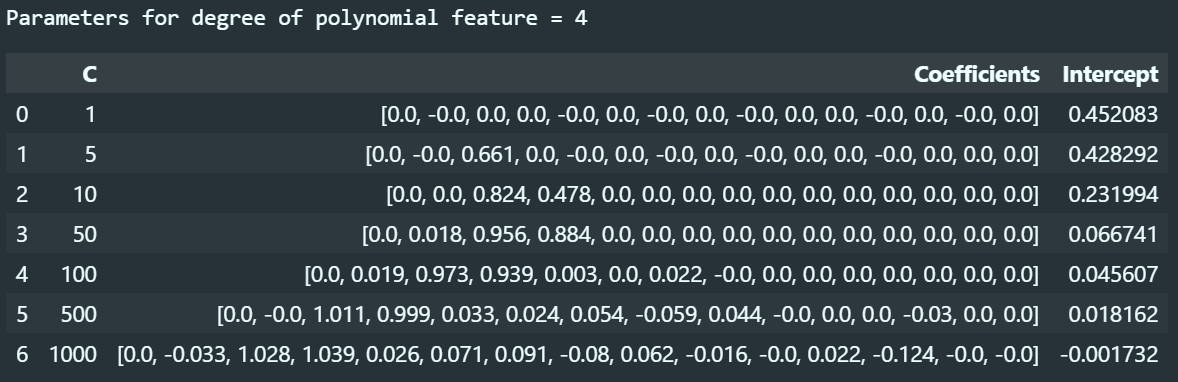
\includegraphics[scale=0.4]{./images/Table_4.png}
  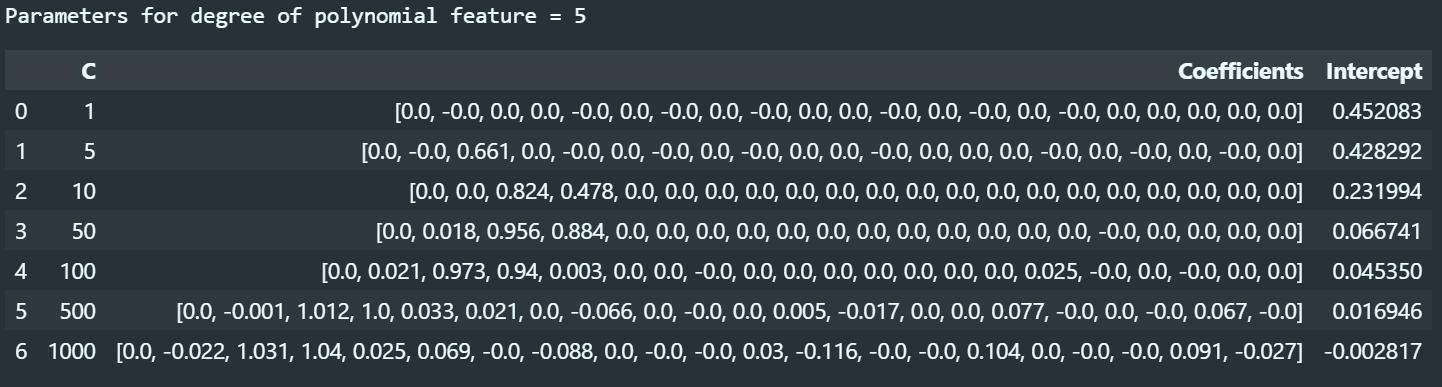
\includegraphics[scale=0.4]{./images/Table_5.png}
\end{center}

\textbf{Explanation of the parameter values calculated(in code):}
The Coefficients mentioned in the middle coloumn of the images above are the coefficients of the Lasso Model mentioned in the middle coloumn of Table 1.
\begin{table}[H]
  \begin{center}
    \caption{\textbf{Lasso models of polynomial feature degree 5 for varying penalty term C.} }
    \begin{tabular}{ |c|c|c|c| }
      \hline
      C    & Intercept & Lasso Model                                                                                                                                                                                                                                        & Lasso Model Coefficients                                \\
      \hline
      1    & 0.452083  & $\begin{aligned}1 + \theta_{1}x_{1} + \theta_{2}x_{2} + \theta_{3}x_{1}^{2}+ \theta_{4}x_{1}x_{2}+\\\nonumber \theta_{5}x_{2}^{2}\\\nonumber+\dots \theta_{19}x_{1}^{5}+ \theta_{20}x_{1}x_{2}^{4}+ \\\nonumber \theta_{21}x_{2}^{5}\end{aligned}$ & \makecell{0.0, -0.0, 0.0, 0.0, -0.0, 0.0, -0.0,         \\0.0, -0.0, 0.0, 0.0, -0.0, 0.0, -0.0, \\0.0, -0.0, 0.0, 0.0, 0.0, 0.0, 0.0} \\
      \hline
      5    & 0.428292  & $\begin{aligned}1 + \theta_{1}x_{1} + \theta_{2}x_{2} + \theta_{3}x_{1}^{2}+ \theta_{4}x_{1}x_{2}+\\\nonumber \theta_{5}x_{2}^{2}\\\nonumber+\dots \theta_{19}x_{1}^{5}+ \theta_{20}x_{1}x_{2}^{4}+ \\\nonumber \theta_{21}x_{2}^{5}\end{aligned}$ & \makecell{0.0, -0.0, 0.661, 0.0, -0.0, 0.0, -0.0,       \\0.0, -0.0, 0.0, 0.0, -0.0, 0.0, 0.0, \\0.0, -0.0, 0.0, -0.0, 0.0, -0.0, 0.0} \\
      \hline
      10   & 0.231994  & $\begin{aligned}1 + \theta_{1}x_{1} + \theta_{2}x_{2} + \theta_{3}x_{1}^{2}+ \theta_{4}x_{1}x_{2}+\\\nonumber \theta_{5}x_{2}^{2}\\\nonumber+\dots \theta_{19}x_{1}^{5}+ \theta_{20}x_{1}x_{2}^{4}+ \\\nonumber \theta_{21}x_{2}^{5}\end{aligned}$ & \makecell{0.0, 0.0, 0.824, 0.478, 0.0, 0.0, 0.0,        \\0.0, 0.0, 0.0, 0.0, 0.0, 0.0, 0.0, \\0.0, 0.0, 0.0, 0.0, 0.0, 0.0, 0.0} \\
      \hline
      50   & 0.066741  & $\begin{aligned}1 + \theta_{1}x_{1} + \theta_{2}x_{2} + \theta_{3}x_{1}^{2}+ \theta_{4}x_{1}x_{2}+\\\nonumber \theta_{5}x_{2}^{2}\\\nonumber+\dots \theta_{19}x_{1}^{5}+ \theta_{20}x_{1}x_{2}^{4}+ \\\nonumber \theta_{21}x_{2}^{5}\end{aligned}$ & \makecell{0.0, 0.018, 0.956, 0.884, 0.0, 0.0, 0.0,      \\0.0, 0.0, 0.0, 0.0, 0.0, 0.0, 0.0, \\0.0, 0.0, -0.0, 0.0, 0.0, 0.0, 0.0} \\
      \hline
      100  & 0.045350  & $\begin{aligned}1 + \theta_{1}x_{1} + \theta_{2}x_{2} + \theta_{3}x_{1}^{2}+ \theta_{4}x_{1}x_{2}+\\\nonumber \theta_{5}x_{2}^{2}\\\nonumber+\dots \theta_{19}x_{1}^{5}+ \theta_{20}x_{1}x_{2}^{4}+ \\\nonumber \theta_{21}x_{2}^{5}\end{aligned}$ & \makecell{0.0, 0.021, 0.973, 0.94, 0.003, 0.0, 0.0,     \\-0.0, 0.0, 0.0, 0.0, 0.0, 0.0, 0.0, \\0.0, 0.025, -0.0, 0.0, -0.0, 0.0, 0.0} \\
      \hline
      500  & 0.016946  & $\begin{aligned}1 + \theta_{1}x_{1} + \theta_{2}x_{2} + \theta_{3}x_{1}^{2}+ \theta_{4}x_{1}x_{2}+\\\nonumber \theta_{5}x_{2}^{2}\\\nonumber+\dots \theta_{19}x_{1}^{5}+ \theta_{20}x_{1}x_{2}^{4}+ \\\nonumber \theta_{21}x_{2}^{5}\end{aligned}$ & \makecell{0.0, -0.001, 1.012, 1.0, 0.033, 0.021, 0.0,   \\-0.066, 0.0, -0.0, 0.0, 0.005, -0.017, 0.0, \\0.0, 0.077, -0.0, 0.0, -0.0, 0.067, -0.0} \\
      \hline
      1000 & -0.002817 & $\begin{aligned}1 + \theta_{1}x_{1} + \theta_{2}x_{2} + \theta_{3}x_{1}^{2}+ \theta_{4}x_{1}x_{2}+\\\nonumber \theta_{5}x_{2}^{2}\\\nonumber+\dots \theta_{19}x_{1}^{5}+ \theta_{20}x_{1}x_{2}^{4}+ \\\nonumber \theta_{21}x_{2}^{5}\end{aligned}$ & \makecell{0.0, -0.022, 1.031, 1.04, 0.025, 0.069, -0.0, \\-0.088, 0.0, -0.0, -0.0, 0.03, -0.116, -0.0, \\-0.0, 0.104, 0.0, -0.0, -0.0, 0.091, -0.027} \\
      \hline
    \end{tabular}
  \end{center}
\end{table}

As C is increased, the number of parameters affecting the Lasso Regression model increase. Thus, the chances of over-fitting increases.

\subsection*{Part c}
\textbf{For each of the models from (b) generate predictions for the target variable.
  Generate these predictions on a grid of feature values. This grid should extend beyond the range of values in the dataset e.g. if the
  first feature in the dataset has values from 0 to 2 generate predictions for values
  from -5 to 5 or thereabouts. Plot these predictions on a 3D data plot and also
  show the training data. Adjust the grid range used for the predictions so that the
  training data can still be clearly seen in the plot. Its up to you to decide how best
  to plot this data but do try to make your plot easy to read (suggestion: it can
  be helpful to plot the predictions as a surface using the matplotlib plot surface
  command and the training data as points using the matplotlib scatter command,
  be sure to add a legend to identify the different curves). With reference to this
  plot discuss how the predictions change as C is varied.}

\begin{figure}[H]
  \begin{center}
    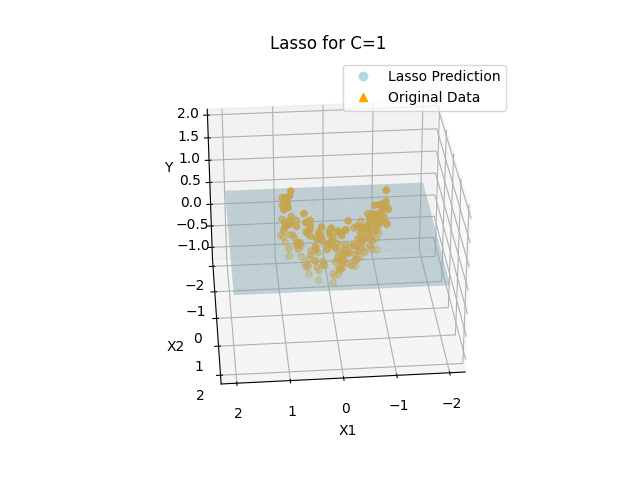
\includegraphics[scale=0.4]{./images/Figure_2_1.png}
    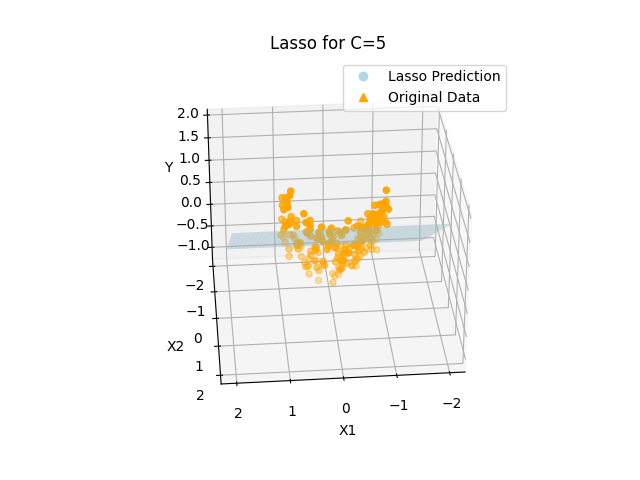
\includegraphics[scale=0.4]{./images/Figure_2_5.png}
    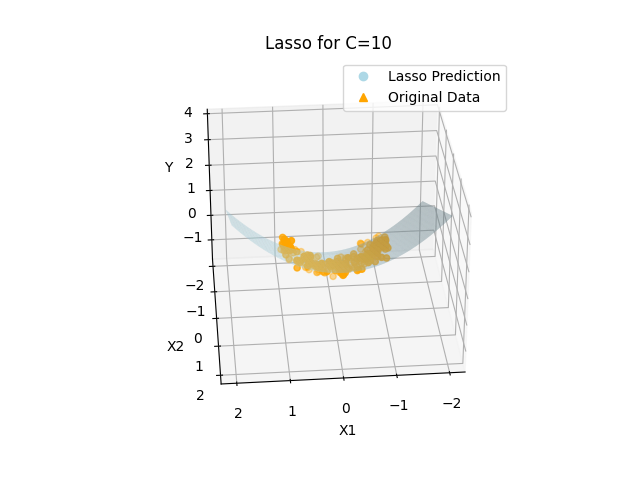
\includegraphics[scale=0.4]{./images/Figure_2_10.png}
    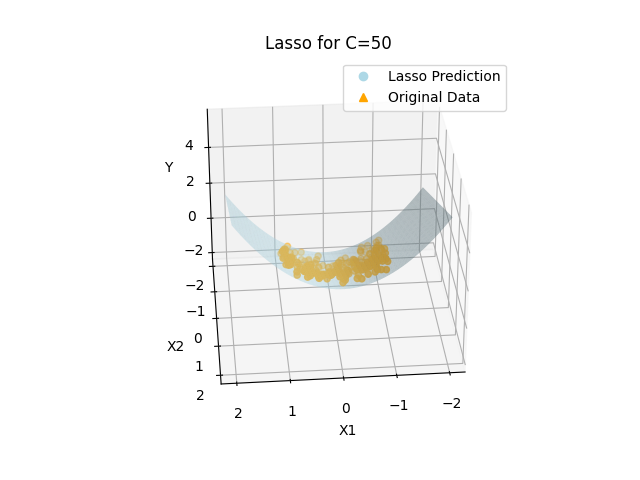
\includegraphics[scale=0.4]{./images/Figure_2_50.png}
    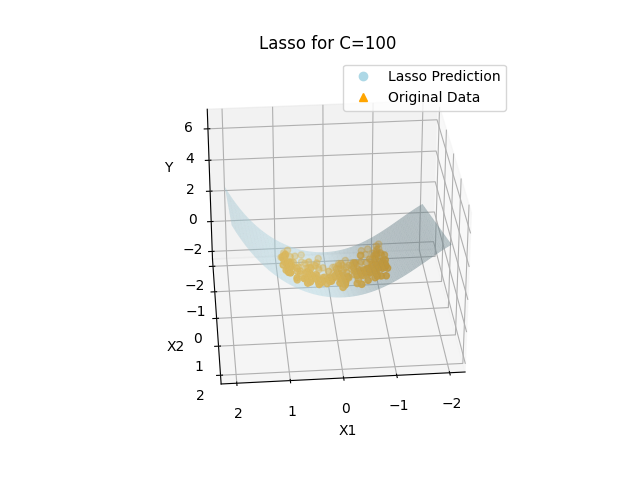
\includegraphics[scale=0.4]{./images/Figure_2_100.png}
    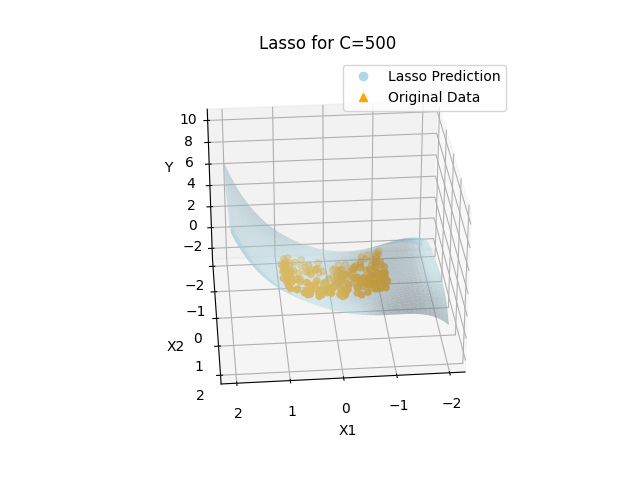
\includegraphics[scale=0.4]{./images/Figure_2_500.png}
    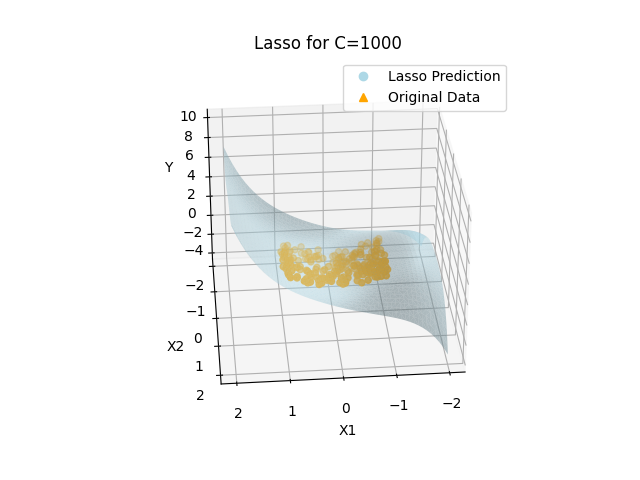
\includegraphics[scale=0.4]{./images/Figure_2_1000.png}
    \caption{a-g: Lasso Regression Predictions for C = [1, 5, 10, 50, 100,500,1000]}
  \end{center}
\end{figure}
For plotting the above plots, I have used matplotlib package's scatter plot to plot the data and tri\_surf to plot the predictions.

Taking into consideration plots 2a-2g, we can observe that on increasing the values of C, the regression model progressively becomes more complex. Thus, providing a better fit for the data. Part (b) states this in a clearer manner. Point to be noted is that, in plot 2(a) and 2(b), we can notice that the regression model is 'under-fitting', meaning that the model is not able to fully fit the data. Whereas, in plot 2(f) and 2(g), we can observe that the model is 'over-fitting', meaning the model is overly compensating for fitting the data.

\subsection*{Part d}
\textbf{What is under- and over-fitting? Using your parameter data from (b) and
  visualisation from (c) explain how penalty weight parameter C can be used to
  manage to trade-off between under- and over-fitting the data.}

\textbf{Underfitting:} refers to when a predictive regression model fails to capture
neither the training data nor generalizes to the new data because it its
often too simple. An underfitting model will not be a suitable one as it
will have poor performance on the training data and the predicted data.
Such a model often shows high bias and low variance.

\textbf{Overfitting:} refers to when a predictive regression model captures the
noise in the data and fits the training data too precisely to such an
extent that it has negative impact as it is unable to fir the new predicted data.
The noise in the training data are picked up by the model and understood as concepts.
These concepts seldom apply to the new predicted data. Hence, it negatively impacts
the model's performance. Such a model often shows low bias and high variance.

\textbf{Trade-Off:} The penalty parameter can be used to achieve a trade-off between
under-fitting and over-fitting of the data by the regression model. From Figure 2(a)[C=1]
and 2(b)[C=5], it is evident that the model is under-fitting as the model is too simple
and is unable to fit all the data. The model is constant in the form of a plane with the
intercept to be 0.452083 and 0.428292 respectively. Hence, the model fails to fit the
non-linear relationship in X1, X2 and y features. Whereas, in Figure 2(f)[C=500] and 2(g)[C=1000],
we can observe that the model is extremely complex and ends up over-fitting the data.
As observed from Table 1, the models contain 10 and 11 polynomial features respectively,
upto degree 5 resulting in a very complex model.
The best trade off between over-fitting and under-fitting is achieved when C values range
between 10 to 100. These are clearly visible in Figure 1(c)[C=50] 1(d)[C=50] 1(e)[C=100].

\subsection*{Part e}
\textbf{Repeat (b)-(c) for a Ridge Regression model. This uses an L2 penalty instead of
  an L1 penalty in the cost function. Compare the impact on the model parameters
  of changing C with Lasso Regression and with Ridge Regression.}

\begin{center}
  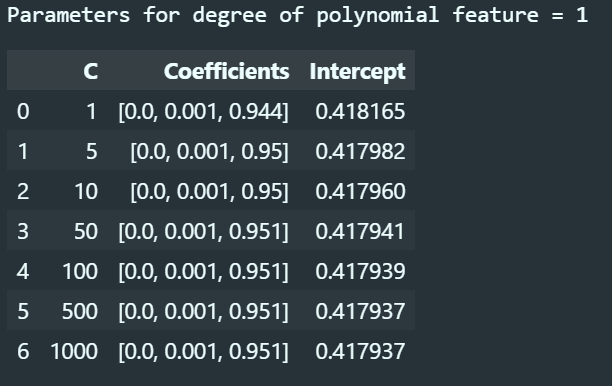
\includegraphics[scale=0.4]{./images/Table_6.png}
  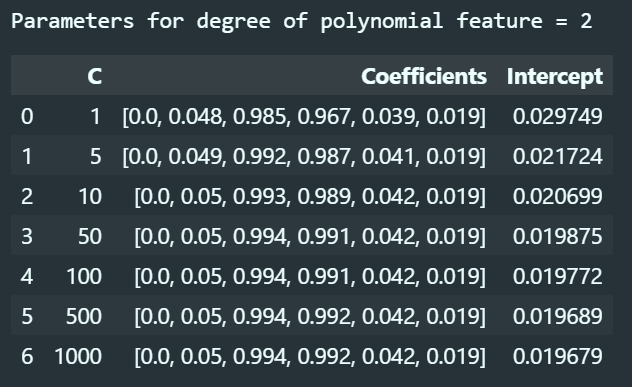
\includegraphics[scale=0.4]{./images/Table_7.png}
  \vspace{5mm}
  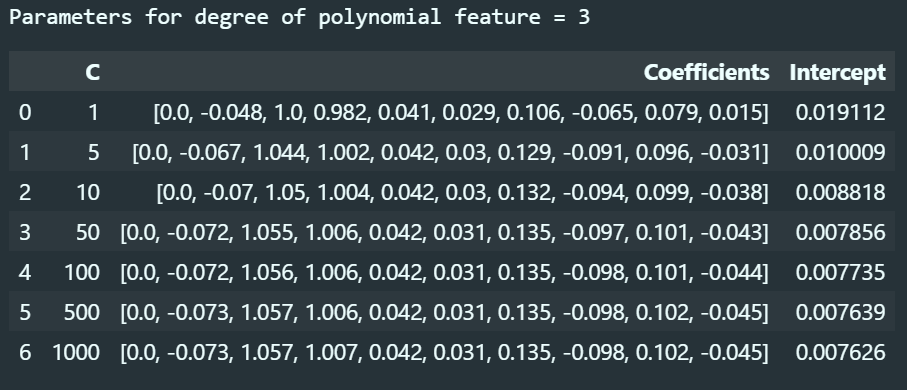
\includegraphics[scale=0.4]{./images/Table_8.png}
  \vspace{5mm}
  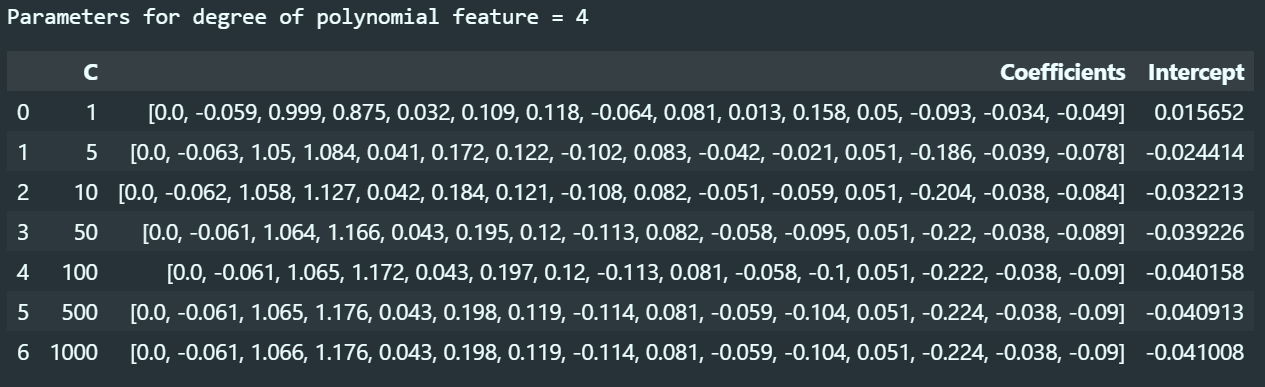
\includegraphics[scale=0.4]{./images/Table_9.png}
  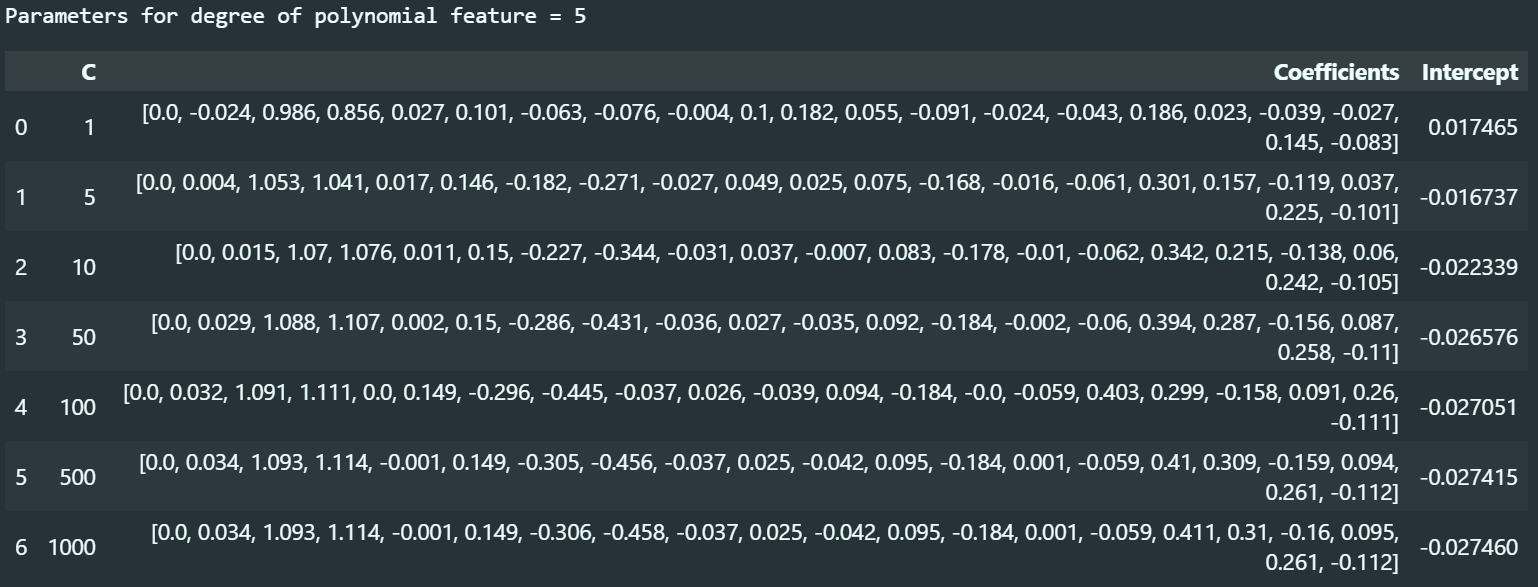
\includegraphics[scale=0.4]{./images/Table_10.png}
\end{center}
\textbf{Explanation of the parameter values calculated(in code):}
The Coefficients mentioned in the middle coloumn of the images above are the coefficients of the Ridge Model mentioned in the middle coloumn of Table 2.
\begin{table}[H]
  \begin{center}
    \caption{\textbf{Ridge models of polynomial feature degree 5 for varying penalty term C.} }
    \begin{tabular}{ |c|c|c|c| }
      \hline
      C    & Intercept & Ridge Model                                                                                                                                                                                                                                        & Ridge Model Coefficients                                   \\
      \hline
      1    & 0.017465  & $\begin{aligned}1 + \theta_{1}x_{1} + \theta_{2}x_{2} + \theta_{3}x_{1}^{2}+ \theta_{4}x_{1}x_{2}+\\\nonumber \theta_{5}x_{2}^{2}\\\nonumber+\dots \theta_{19}x_{1}^{5}+ \theta_{20}x_{1}x_{2}^{4}+ \\\nonumber \theta_{21}x_{2}^{5}\end{aligned}$ & \makecell{0.0, -0.024, 0.986, 0.856, 0.027, 0.101, -0.063, \\-0.076, -0.004, 0.1, 0.182, 0.055, -0.091, -0.024, \\-0.043, 0.186, 0.023, -0.039, -0.027, 0.145, -0.083} \\
      \hline
      5    & -0.016737 & $\begin{aligned}1 + \theta_{1}x_{1} + \theta_{2}x_{2} + \theta_{3}x_{1}^{2}+ \theta_{4}x_{1}x_{2}+\\\nonumber \theta_{5}x_{2}^{2}\\\nonumber+\dots \theta_{19}x_{1}^{5}+ \theta_{20}x_{1}x_{2}^{4}+ \\\nonumber \theta_{21}x_{2}^{5}\end{aligned}$ & \makecell{0.0, 0.004, 1.053, 1.041, 0.017, 0.146, -0.182,  \\-0.271, -0.027, 0.049, 0.025, 0.075, -0.168, -0.016, \\-0.061,0.301, 0.157, -0.119, 0.037, 0.225, -0.101} \\
      \hline
      10   & -0.022339 & $\begin{aligned}1 + \theta_{1}x_{1} + \theta_{2}x_{2} + \theta_{3}x_{1}^{2}+ \theta_{4}x_{1}x_{2}+\\\nonumber \theta_{5}x_{2}^{2}\\\nonumber+\dots \theta_{19}x_{1}^{5}+ \theta_{20}x_{1}x_{2}^{4}+ \\\nonumber \theta_{21}x_{2}^{5}\end{aligned}$ & \makecell{0.0, 0.015, 1.07, 1.076, 0.011, 0.15, -0.227,    \\-0.344, -0.031, 0.037, -0.007, 0.083, -0.178, -0.01, \\-0.062, 0.342, 0.215, -0.138, 0.06, 0.242, -0.105} \\
      \hline
      50   & -0.026576 & $\begin{aligned}1 + \theta_{1}x_{1} + \theta_{2}x_{2} + \theta_{3}x_{1}^{2}+ \theta_{4}x_{1}x_{2}+\\\nonumber \theta_{5}x_{2}^{2}\\\nonumber+\dots \theta_{19}x_{1}^{5}+ \theta_{20}x_{1}x_{2}^{4}+ \\\nonumber \theta_{21}x_{2}^{5}\end{aligned}$ & \makecell{0.0, 0.029, 1.088, 1.107, 0.002, 0.15, -0.286,   \\-0.431, -0.036, 0.027, -0.035, 0.092, -0.184, -0.002, \\-0.06, 0.394, 0.287, -0.156, 0.087, 0.258, -0.11} \\
      \hline
      100  & -0.027051 & $\begin{aligned}1 + \theta_{1}x_{1} + \theta_{2}x_{2} + \theta_{3}x_{1}^{2}+ \theta_{4}x_{1}x_{2}+\\\nonumber \theta_{5}x_{2}^{2}\\\nonumber+\dots \theta_{19}x_{1}^{5}+ \theta_{20}x_{1}x_{2}^{4}+ \\\nonumber \theta_{21}x_{2}^{5}\end{aligned}$ & \makecell{0.0, 0.032, 1.091, 1.111, 0.0, 0.149, -0.296,    \\-0.445, -0.037, 0.026, -0.039, 0.094, -0.184, -0.0, \\-0.059, 0.403, 0.299, -0.158, 0.091, 0.26, -0.111} \\
      \hline
      500  & -0.027415 & $\begin{aligned}1 + \theta_{1}x_{1} + \theta_{2}x_{2} + \theta_{3}x_{1}^{2}+ \theta_{4}x_{1}x_{2}+\\\nonumber \theta_{5}x_{2}^{2}\\\nonumber+\dots \theta_{19}x_{1}^{5}+ \theta_{20}x_{1}x_{2}^{4}+ \\\nonumber \theta_{21}x_{2}^{5}\end{aligned}$ & \makecell{0.0, 0.034, 1.093, 1.114, -0.001, 0.149, -0.305, \\-0.456, -0.037, 0.025, -0.042, 0.095, -0.184, 0.001, \\-0.059, 0.41, 0.309, -0.159, 0.094, 0.261, -0.112} \\
      \hline
      1000 & -0.027460 & $\begin{aligned}1 + \theta_{1}x_{1} + \theta_{2}x_{2} + \theta_{3}x_{1}^{2}+ \theta_{4}x_{1}x_{2}+\\\nonumber \theta_{5}x_{2}^{2}\\\nonumber+\dots \theta_{19}x_{1}^{5}+ \theta_{20}x_{1}x_{2}^{4}+ \\\nonumber \theta_{21}x_{2}^{5}\end{aligned}$ & \makecell{0.0, 0.034, 1.093, 1.114, -0.001, 0.149, -0.306, \\-0.458, -0.037, 0.025, -0.042, 0.095, -0.184, 0.001, \\-0.059, 0.411, 0.31, -0.16, 0.095, 0.261, -0.112} \\
      \hline
    \end{tabular}
  \end{center}
\end{table}

As C is increased, the number of parameters affecting the Ridge Regression model increase. Thus, the chances of over-fitting increases.

\begin{figure}[H]
  \begin{center}
    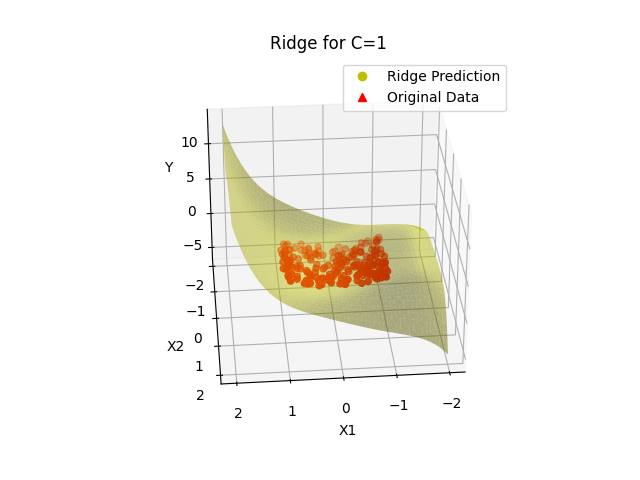
\includegraphics[scale=0.4]{./images/Figure_3_1.png}
    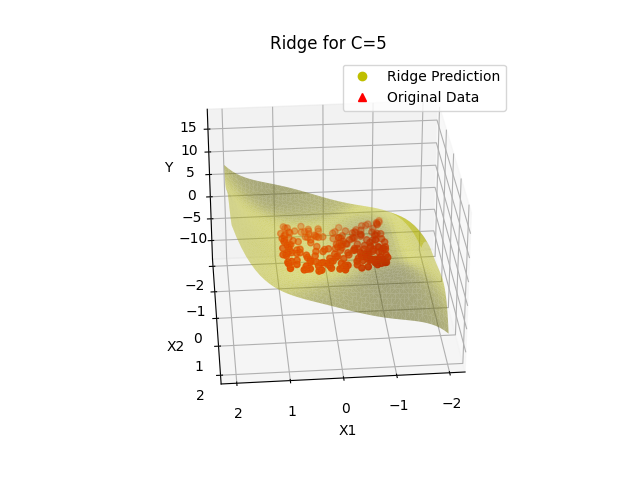
\includegraphics[scale=0.4]{./images/Figure_3_5.png}
    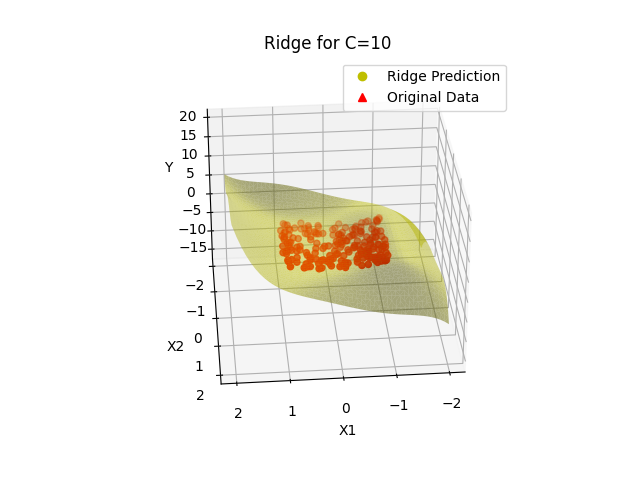
\includegraphics[scale=0.4]{./images/Figure_3_10.png}
    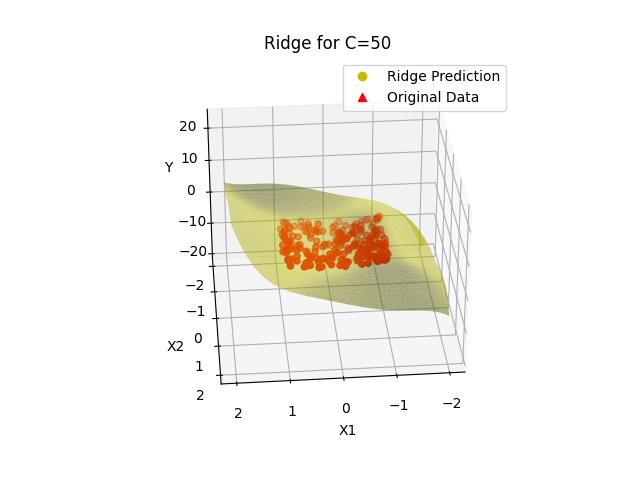
\includegraphics[scale=0.4]{./images/Figure_3_50.png}
    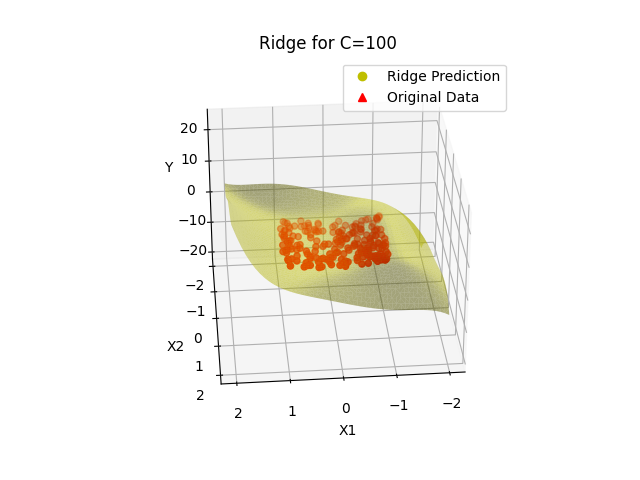
\includegraphics[scale=0.4]{./images/Figure_3_100.png}
    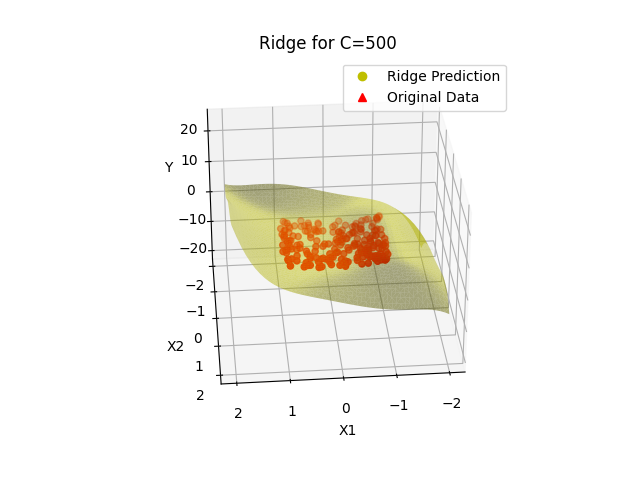
\includegraphics[scale=0.4]{./images/Figure_3_500.png}
    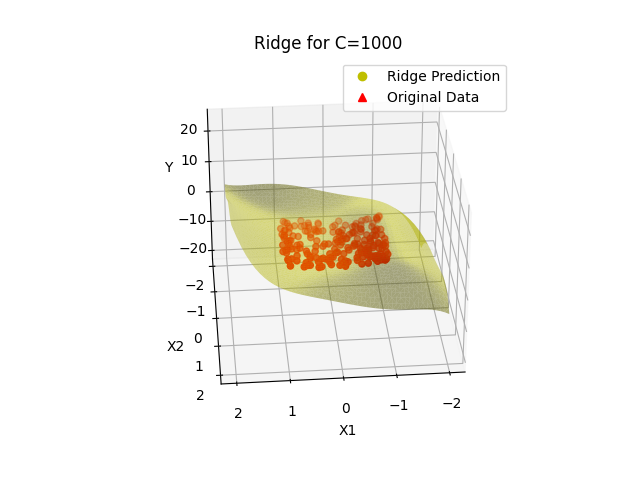
\includegraphics[scale=0.4]{./images/Figure_3_1000.png}
    \caption{a-g: Ridge Regression Predictions for C = [1, 5, 10, 50, 100,500,1000]}
  \end{center}
\end{figure}

In the same way as Lasso Regression models were trained, Ridge regression models were trained on the data set provided along with the polynomial features equal
to all combinations of powers of the two features up to power 5. I used PolynomialFeatures function from sklearn package.
Ridge regression models were trained on the data for a large number of penalty values, specifically, [1, 5, 10, 50, 100, 500,
    1000] values.

As observed from the plots above, it can be observed that the plot 3(a) fits the data. As C is inversely proportional to the penalty parameter, as we increase the C value, the model becomes exponentially more complex by morphs to fit the data. All the models in plot 3(b) to 3(g), 'over-fit' the data.

\section*{Question ii}
\textbf{Using the Lasso model with polynomial features from (i) you’ll now look at using
  cross-validation to select C.}

\subsection*{Part a}
\textbf{Use 5-fold cross-validation to plot the mean and standard deviation of the prediction error vs C. Use the matplotlib errorbar function for this. You will need
  to choose the range of values of C to plot, justify your choice.}



\begin{figure}[hbt!]
  \begin{center}
    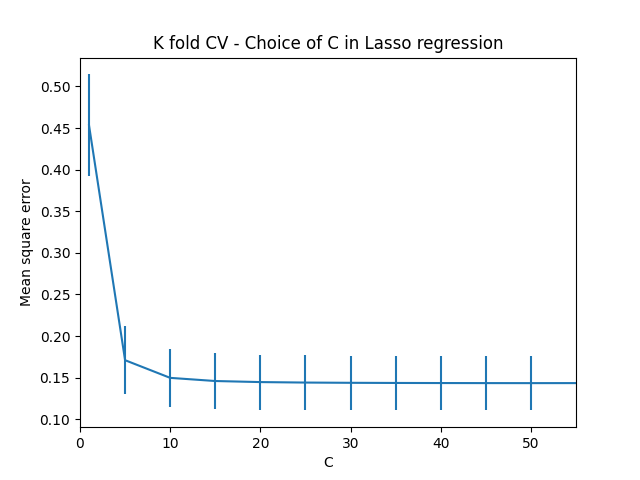
\includegraphics[scale=0.4]{./images/Figure_4.png}
    \caption{k-Fold Cross Validation - Choice of C}
  \end{center}
\end{figure}

The optimal value of the penalty term, C in Lasso Regression Model, was determined by k-fold
cross-validation, where k was deemed to be 5. For each value of C, the penalty term, the k-fold
cross-validation was implemented to determine the model performance. The performance was estimated
based on the mean and the standard deviation of the prediction vs C.
The model was tested on the following range of C values = [1,5,10,15,20,25,30,35,40,45,50]. As per
the rule of thumb, the most common C values selected are 1,5,10.... I did not deviate from the norm.
I also checked the MSE for  higher values such as 100, 500, and 1000.


As observed in Figure 4(a), the Mean Square Error(MSE) is the maximum when the penalty term is lowest.
The MSE keeps on decreaing till the penalty value is 10. For penalty values ranging from 10 to 1000, we
can observe that the net change in MSE is negligible.

\subsection*{Part b}
\textbf{Based on the cross-validation data what value of C would you recommend be
  used here? Importantly, explain the reasons for your choice.}

From Figure 4, we can observe that the Mean Square Error(MSE) is inversely proportional
to the penalty term in the range 0 to 10. As we keep on increasing the penalty term value,
we can note that the net change in the MSE is negligible. Thus, any value for penalty term
in the range 10 to 1000 can be chosen as the performance is the highest when the MSE is lowest.

\subsection*{Part c}
\textbf{ Repeat (b)-(c) for a Ridge Regression model}
\begin{figure}[H]
  \begin{center}
    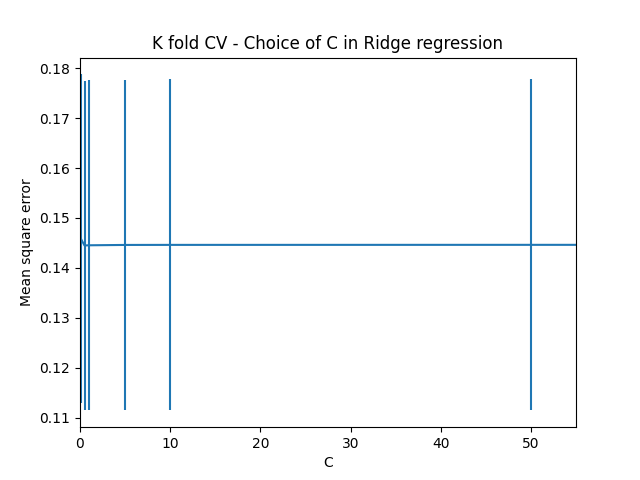
\includegraphics[scale=0.4]{./images/Figure_5.png}
    \caption{k-Fold Cross Validation - Choice of C}
  \end{center}
\end{figure}

The optimal value of the penalty term, C in Ridge Regression Model, was determined by k-fold
cross-validation, where k was deemed to be 5. For each value of C, the penalty term, the k-fold
cross-validation was implemented to determine the model performance. The performance was estimated
based on the mean and the standard deviation of the prediction vs C.
The model was tested on the following range of C values = [0.1, 0.5, 1, 5, 10, 50, 100]. I chose
these values as in Ridge Regression Model, the change in MSE was not visible otherwise.

From Figure 5, we can observe that the Mean Square Error(MSE) is inversely proportional
to the penalty term in the range 0 to 0.5. As we keep on increasing the penalty term value,
we can note that the net change in the MSE is negligible. Thus, any value for penalty term
in the range 1 to 50 can be chosen as the performance is the highest when the MSE is lowest.


\section*{Appendix}
\textbf{Imports:}
\begin{lstlisting}[language=Python]
  #Imports:
  import pandas as pd
  import numpy as np
  import matplotlib.pyplot as plt
  from mpl_toolkits.mplot3d import Axes3D
  from sklearn.preprocessing import PolynomialFeatures
  from sklearn import model_selection
  from sklearn.linear_model import Ridge
  from sklearn.linear_model import Lasso
  import matplotlib as mtplt
  from sklearn.model_selection import KFold
  from sklearn.model_selection import train_test_split
  from sklearn.metrics import mean_squared_error
  from math import sqrt
\end{lstlisting}
\textbf{Question i a:}
\begin{lstlisting}[language=Python]
  fig=plt.figure()
  ax= fig.add_subplot(111,projection='3d')
  ax.scatter(X1,X2,y)
  ax.set_xlabel('X1')
  ax.set_ylabel('X2')
  ax.set_zlabel('Y')
  ax.set_title('# id:15-15-15 ')
  # ax.view_init(180)
  # ax.view_init(360)
  # plt.savefig('LaTex/images/Figure_1.png')
  # plt.savefig('LaTex/images/Figure_1_180.png')
  # plt.savefig('LaTex/images/Figure_1_360.png')
  plt.show()
  marks=[]
  for val in point:
    marks.append(val)
  center = np.mean(marks, axis=0)
  _, e_values, e_vectors = np.linalg.svd(marks - center, full_matrices=False)
  normal = e_vectors[2]
  dispersion = e_values[2]
  print('normal: ',normal)
  print('dispersion: ',dispersion)
\end{lstlisting}
\textbf{Question i b:}
\begin{lstlisting}[language=Python]
  def get_regression_model_values_by_type(x,y,degree_poly,test_c_vals,name_of_model):
  
  x_poly=PolynomialFeatures(degree_poly).fit_transform(x)
  
  results_df=[]

  for c in test_c_vals:
    if(name_of_model=='Lasso'):
      model=Lasso(alpha=1/(2*c))
    elif (name_of_model=='Ridge'):
      model=Ridge(alpha=1/(2*c))
  
    model.fit(x_poly,y)

    result_dict={
      'C': c,
      'Coefficients':np.around(model.coef_,decimals=3),
      'Intercept': model.intercept_
    }

    results_df.append(result_dict)
  
  model_results=pd.DataFrame(results_df)
  return model_results

# poly_feature=5
test_c_values=[1, 5, 10, 50, 100,500,1000]
model_name='Lasso'
range_of_poly=[1,2,3,4,5]
poly_feature=5
for i in range_of_poly:
  result=get_regression_model_values_by_type(X,y,i,test_c_values,model_name)
  with pd.option_context('display.max_colwidth', 400):
    print(f'Parameters for degree of polynomial feature = {i}')
    display(result)
\end{lstlisting}
\textbf {Question i c:}
\begin{lstlisting}[language=Python]
  def plot_preds_by_c_and_model(x,y,x_test,test_c_values,model_name,colour_of_plot):

  x_poly=PolynomialFeatures(poly_feature).fit_transform(x)
  x_poly_test =PolynomialFeatures(poly_feature).fit_transform(x_test)

  for c in test_c_values:
    if(model_name=='Lasso'):
        model=Lasso(alpha=1/(2*c))
    elif (model_name=='Ridge'):
        model=Ridge(alpha=1/(2*c))

    model.fit(x_poly,y)
    predictions=model.predict(x_poly_test)
    

    fig=plt.figure()
    ax=fig.add_subplot(111,projection='3d')

    ax.plot_trisurf(x_test[:,0],x_test[:,1],predictions,color=colour_of_plot[0],alpha=0.5)
    ax.scatter(X1,X2,y,color=colour_of_plot[1], label='Original Data')
    colors=['y','r']
    ax.set_xlabel('X1')
    ax.set_ylabel('X2')
    ax.set_zlabel('Y')
    ax.set_title(f'{model_name} for C={c}')

    scatter_plot_1=mtplt.lines.Line2D([0],[0],linestyle='none',c=colour_of_plot[0],marker='o')
    scatter_plot_2=mtplt.lines.Line2D([0],[0],linestyle='none',c=colour_of_plot[1],marker='^')
    ax.legend([scatter_plot_1,scatter_plot_2],[f'{model_name} Prediction','Original Data'],numpoints=1)
    ax.view_init(azim=85)
    if model_name=='Lasso':
      plt.savefig(f'LaTex/images/Figure_2_{c}.png')
    elif model_name=='Ridge':
      plt.savefig(f'LaTex/images/Figure_3_{c}.png')

poly_test_degree = 5 
test_c = [1, 5, 10, 50, 100,500,1000]
model_type = 'Lasso'
plot_colours=['lightblue','orange']
Xtest=[]
grid=np.linspace(-2,2)
for i in grid:
  for j in grid:
      Xtest.append([i,j])
Xtest = np.array(Xtest)

plot_preds_by_c_and_model(X,y,Xtest,test_c,model_type,plot_colours)
\end{lstlisting}
\textbf{Question i e:}
\begin{lstlisting}[language=Python]
  #Get Regression results
range_of_poly = [1,2,3,4,5] 
for i in range_of_poly:
    c_test = [1, 5, 10, 50, 100,500,1000]
    model_type = 'Ridge'
    result=get_regression_model_values_by_type(X, y, i, c_test, model_type)
    with pd.option_context('display.max_colwidth', 400):
        print(f'Parameters for degree of polynomial feature = {i}')
        display(result)

#Plot Predictions 
model_type = 'Ridge'
plot_colors = ['y', 'r']
plot_preds_by_c_and_model(X, y, Xtest, c_test, model_type, plot_colors)
\end{lstlisting}
\textbf{Question ii a:}
\begin{lstlisting}[language=Python]
  def kfcv(x,y,c_range,name_of_model):
  mean_error=[];std_error=[];
  for c in c_range:
    if(name_of_model=='Lasso'):
      model=Lasso(alpha=1/(2*c))
    elif(name_of_model=='Ridge'):
      model=Ridge(alpha=1/(2*c))
    
    mean_square_error_temp=[]
    kf=KFold(n_splits=5)
    for train,test in kf.split(x):
      model.fit(x[train],y[train])
      predictions=model.predict(x[test])
      mean_square_error_temp.append(mean_squared_error(y[test],predictions))
    mean_error.append(np.array(mean_square_error_temp).mean())
    std_error.append(np.array(mean_square_error_temp).std())
  plt.errorbar(c_range,mean_error,yerr=std_error)
  plt.xlabel('C'); plt.ylabel('Mean square error')
  plt.title('K fold CV - Choice of C in {} regression'.format(name_of_model))
  plt.xlim((0,55))
  if name_of_model=='Lasso':
    plt.savefig(f'LaTex/images/Figure_4.png')
  elif name_of_model=='Ridge':
    plt.savefig(f'LaTex/images/Figure_5.png')
  plt.show()

c_vals=[1,5,10,15,20,25,30,35,40,45,50,100,500,1000]
model='Lasso'
kfcv(X,y,c_vals,model)

c_vals_1=[0.1, 0.5, 1, 5, 10, 50, 100]
model1='Ridge'
kfcv(X,y,c_vals_1,model1)
\end{lstlisting}
\end{document}